\documentclass[11pt]{article}

\usepackage[a4paper,margin=1in]{geometry}
\usepackage{amsmath, amssymb}
\usepackage{array}
\usepackage{booktabs}
\usepackage{caption}
\usepackage{enumitem}
\usepackage{float}
\usepackage{graphicx}
\usepackage{hyperref}
\usepackage{longtable}
\usepackage{parskip}
\usepackage{tabularx}
\usepackage{xcolor}

\IfFileExists{generated_results.tex}{\newcommand{\MNISTTestAcc}{98.76\%}
\newcommand{\CMNISTBiasedAcc}{98.49\%}
\newcommand{\CMNISTUnbiasedAcc}{75.52\%}
\newcommand{\STLTestAcc}{79.61\%}
\newcommand{\STLStatus}{Completed}
\newcommand{\MNISTParamCount}{42722}
\newcommand{\CMNISTParamCount}{42866}
\newcommand{\ToyOutput}{2.500}
\newcommand{\ToyLoss}{0.125}
\newcommand{\ToyResidualOutput}{2.000}
\newcommand{\ToyResidualLoss}{0.500}
\newcommand{\MNISTGeneralization}{The model generalizes well: training accuracy (0.982) and validation accuracy (0.986) stay close, with an absolute gap of 0.003.}
\newcommand{\FilterInterpretation}{Filter 1 emphasizes vertical edge / stroke transitions with a bright-center bias; Filter 2 emphasizes vertical edge / stroke transitions with a dark-center / contrast bias; Filter 3 emphasizes horizontal edge / stroke transitions with a dark-center / contrast bias; Filter 4 emphasizes horizontal edge / stroke transitions with a bright-center bias.}
}{}

\hypersetup{
  colorlinks=true,
  linkcolor=blue!50!black,
  urlcolor=blue!60!black
}

\setlist[itemize]{leftmargin=1.4em, itemsep=0.25em, topsep=0.3em}
\renewcommand{\arraystretch}{1.2}

\newcommand{\StudentName}{Muhammad Abdullah}
\newcommand{\RollNumber}{25280050}
\newcommand{\RepoURL}{https://github.com/abdull2325/assignment3-dl}
\newcommand{\SubmissionDate}{8 April 2026}

\begin{document}

\begin{titlepage}
  \centering
  {\large Lahore University of Management Sciences\par}
  {\large School of Science and Engineering\par}
  {\large Department of Electrical Engineering\par}
  \vspace{1.4cm}
  {\huge \textbf{AI600 -- Deep Learning}\par}
  \vspace{0.25cm}
  {\LARGE \textbf{Assignment 3 Report}\par}
  \vspace{1.4cm}

  \begin{tabular}{>{\bfseries}p{0.32\textwidth}p{0.58\textwidth}}
    Student Name & \StudentName \\
    Roll Number & \RollNumber \\
    Semester & Spring 2026 \\
    Submission Date & \SubmissionDate \\
    GitHub Repository & \href{\RepoURL}{\RepoURL} \\
    Local Workspace & \texttt{/Users/abdullah/Downloads/cmnist} \\
  \end{tabular}

  \vfill

  \begin{minipage}{0.9\textwidth}
    \small
    This report contains the required analytical derivations, implementation details,
    measured experimental results, visualizations, model interpretations, and the
    mandatory Generative AI disclosure for AI600 Assignment 3.
  \end{minipage}
\end{titlepage}

\pagenumbering{roman}
\tableofcontents
\newpage
\listoffigures
\newpage
\pagenumbering{arabic}

\section{Submission Overview}

This submission is complete with respect to the assessed portions of the assignment. The
analytical section covers Q1 and Q3 in detail and also includes worked solutions for the
practice-only Q2 and Q4 for completeness. The programming section includes Task 1
(standard MNIST and Colored-MNIST) and Task 2 (transfer learning on STL-10 plus GradCAM
visualization), along with plots, learned filters, and interpretation.

\begin{table}[H]
  \centering
  \caption{Assignment deliverables checklist}
  \small
  \begin{tabular}{p{0.46\textwidth}p{0.14\textwidth}p{0.28\textwidth}}
    \toprule
    Requirement & Status & Evidence \\
    \midrule
    Analytical solutions for required questions & Complete & Sections 2.1 and 2.2 \\
    Custom CNN for MNIST under 50k parameters & Complete & \MNISTParamCount{} parameters \\
    Colored-MNIST bias analysis & Complete & Biased and unbiased accuracies reported \\
    STL-10 transfer learning with frozen backbone & Complete & \STLTestAcc{} test accuracy \\
    GradCAM visualization on correct and incorrect examples & Complete & Figure \ref{fig:stl-gradcam} \\
    Public GitHub repository link on first page & Complete & Title page / overview \\
    Generative AI prompt, output, and edits disclosure & Complete & Section 5 \\
    PDF report and LaTeX source & Complete & Report PDF and LaTeX source included \\
    \bottomrule
  \end{tabular}
\end{table}

\begin{table}[H]
  \centering
  \caption{Experimental performance summary}
  \small
  \begin{tabular}{p{0.31\textwidth}p{0.22\textwidth}p{0.17\textwidth}p{0.16\textwidth}}
    \toprule
    Experiment & Model & Parameters & Accuracy \\
    \midrule
    Standard MNIST & Custom CNN & \MNISTParamCount{} & \MNISTTestAcc \\
    Colored-MNIST biased test & Custom CNN (RGB) & \CMNISTParamCount{} & \CMNISTBiasedAcc \\
    Colored-MNIST unbiased test & Custom CNN (RGB) & \CMNISTParamCount{} & \CMNISTUnbiasedAcc \\
    STL-10 test & Frozen ResNet-18 + linear head & 5130 trainable & \STLTestAcc \\
    \bottomrule
  \end{tabular}
\end{table}

\section{Analytical Part}

\subsection{Q1: Forward and Backward Pass}

The input image and convolution filter are
\[
X=
\begin{bmatrix}
1 & 2 & 0\\
0 & 1 & 1\\
1 & 0 & 2
\end{bmatrix},
\quad
W=
\begin{bmatrix}
1 & 0\\
-1 & 1
\end{bmatrix},
\quad
b=0,
\quad
V=
\begin{bmatrix}
1 & -1 & 2 & 0.5
\end{bmatrix},
\quad
c=1.
\]

\subsubsection*{Q1(a): Forward Pass}

The valid \(2\times2\) patches are:
\[
P_{11}=
\begin{bmatrix}
1 & 2\\
0 & 1
\end{bmatrix},
\quad
P_{12}=
\begin{bmatrix}
2 & 0\\
1 & 1
\end{bmatrix},
\quad
P_{21}=
\begin{bmatrix}
0 & 1\\
1 & 0
\end{bmatrix},
\quad
P_{22}=
\begin{bmatrix}
1 & 1\\
0 & 2
\end{bmatrix}.
\]

Therefore,
\[
z_{11}=2,\quad
z_{12}=2,\quad
z_{21}=-1,\quad
z_{22}=3,
\]
so the pre-activation map is
\[
Z=
\begin{bmatrix}
2 & 2\\
-1 & 3
\end{bmatrix}.
\]

After ReLU,
\[
A=\text{ReLU}(Z)=
\begin{bmatrix}
2 & 2\\
0 & 3
\end{bmatrix}.
\]

Flattening row-wise gives
\[
A_{\text{flat}}=
\begin{bmatrix}
2 & 2 & 0 & 3
\end{bmatrix}^{T}.
\]

The scalar prediction is
\[
Y=V\cdot A_{\text{flat}}+c
=1(2)+(-1)(2)+2(0)+0.5(3)+1
=2.5.
\]

With target \(T=3\), the loss is
\[
L=\frac{1}{2}(Y-T)^2
=\frac{1}{2}(2.5-3)^2
=0.125.
\]

\subsubsection*{Q1(b): Backward Pass}

First,
\[
\frac{\partial L}{\partial Y}=Y-T=2.5-3=-0.5.
\]

Hence,
\[
\frac{\partial L}{\partial V}
=\frac{\partial L}{\partial Y}\,A_{\text{flat}}^{T}
=-0.5
\begin{bmatrix}
2 & 2 & 0 & 3
\end{bmatrix}
=
\begin{bmatrix}
-1 & -1 & 0 & -1.5
\end{bmatrix}.
\]

Next,
\[
\frac{\partial L}{\partial A_{\text{flat}}}
=\frac{\partial L}{\partial Y}V
=-0.5
\begin{bmatrix}
1 & -1 & 2 & 0.5
\end{bmatrix}
=
\begin{bmatrix}
-0.5 & 0.5 & -1 & -0.25
\end{bmatrix}.
\]

Reshaping:
\[
\frac{\partial L}{\partial A}=
\begin{bmatrix}
-0.5 & 0.5\\
-1 & -0.25
\end{bmatrix}.
\]

Because ReLU blocks gradients where \(Z\le 0\),
\[
\frac{\partial L}{\partial Z}
=
\begin{bmatrix}
-0.5 & 0.5\\
0 & -0.25
\end{bmatrix}.
\]

The convolution-filter gradient is the sum of patch contributions:
\[
\frac{\partial L}{\partial W}
=
\left(-0.5\right)P_{11}
+\left(0.5\right)P_{12}
+0\cdot P_{21}
+\left(-0.25\right)P_{22}.
\]

So,
\[
\frac{\partial L}{\partial W}
=
\begin{bmatrix}
0.25 & -1.25\\
0.5 & -0.5
\end{bmatrix}.
\]

\subsubsection*{Q1(c): Interpretation}

The largest-magnitude entry of \(\frac{\partial L}{\partial W}\) is the top-right weight:
\[
\left|\frac{\partial L}{\partial W_{1,2}}\right|=1.25.
\]

Since
\[
\frac{\partial L}{\partial W_{1,2}}=-1.25,
\]
one gradient-descent step updates it as
\[
W_{1,2}\leftarrow W_{1,2}-\eta\frac{\partial L}{\partial W_{1,2}}
=W_{1,2}+1.25\eta,
\]
so this weight increases the most.

Structurally, \(W_{1,2}\) multiplies the top-right pixel inside each active patch. Its gradient becomes large because it sees a large input value \(x_{1,2}=2\) in the first active patch and another positive input in the bottom-right active patch, while both corresponding upstream signals are negative. Those contributions add to a strong negative gradient.

\subsection{Q3: Pooling and Normalization}

\subsubsection*{Q3(a): Global Max Pooling}

Replacing the flattening plus fully-connected layer with global max pooling gives
\[
Y=\max(A)=3.
\]

Since the target is also \(T=3\),
\[
L=\frac{1}{2}(3-3)^2=0.
\]

Therefore, for this specific numeric example, every gradient is zero. In particular, all pixels in \(X\) have zero gradient.

Structurally, global max pooling would normally route gradient only through the maximal activation \(a_{22}\). That activation depends only on the receptive field
\[
\begin{bmatrix}
X_{2,2} & X_{2,3}\\
X_{3,2} & X_{3,3}
\end{bmatrix},
\]
so if the loss were nonzero, only those four pixels could receive gradient.

\subsubsection*{Q3(b): Layer Normalization}

Using the original architecture, the post-ReLU feature map is
\[
A=
\begin{bmatrix}
2 & 2\\
0 & 3
\end{bmatrix}.
\]

Its mean is
\[
\mu=\frac{2+2+0+3}{4}=1.75.
\]

Its variance is
\[
\sigma^2
=\frac{(2-1.75)^2+(2-1.75)^2+(0-1.75)^2+(3-1.75)^2}{4}
=1.1875.
\]

With \(\gamma=1\), \(\beta=0\), and \(\epsilon=0\),
\[
A_{\text{norm}}=\frac{A-\mu}{\sqrt{\sigma^2}}
=
\begin{bmatrix}
0.2294 & 0.2294\\
-1.6059 & 1.1471
\end{bmatrix}.
\]

\subsubsection*{Q3(c): Interpretation}

Global max pooling computes
\[
Y=\max\{a_{11},a_{12},a_{21},a_{22}\}.
\]

If a small translation of the input shifts the strongest local feature from one spatial position to another but preserves the maximum activation value, then the max operator returns the same \(Y\). As a result, the loss remains unchanged. This is the mathematical reason that max pooling provides partial translation invariance.

\subsection{Practice Questions (Worked for Completeness)}

\subsubsection*{Q2(a)--Q2(c): Input Gradient and Perturbation}

From the chain rule,
\[
\frac{\partial L}{\partial X}
=
\begin{bmatrix}
-0.5 & 0.5 & 0\\
0.5 & -1.25 & 0.5\\
0 & 0.25 & -0.25
\end{bmatrix}.
\]

Hence,
\[
\frac{\partial L}{\partial X_{2,2}}=-1.25.
\]

Using the linear approximation
\[
L(X+\epsilon e_{2,2})\approx L(X)+\epsilon\frac{\partial L}{\partial X_{2,2}},
\]
the adversary should choose a negative \(\epsilon\) to increase the loss.

The center pixel has a larger gradient than a corner pixel because it participates in four overlapping convolution windows. Weight sharing reuses the same kernel coefficients at each location, so the total gradient accumulates contributions from multiple spatial paths.

\subsubsection*{Q4(a)--Q4(c): Residual Variant}

The cropped identity is
\[
X_{\text{crop}}=
\begin{bmatrix}
1 & 2\\
0 & 1
\end{bmatrix}.
\]

Therefore,
\[
A_{\text{res}}=A+X_{\text{crop}}=
\begin{bmatrix}
3 & 4\\
0 & 4
\end{bmatrix}.
\]

The new prediction is
\[
Y_{\text{res}}
=1(3)+(-1)(4)+2(0)+0.5(4)+1
=2.
\]

The gradient with respect to the top-left input pixel becomes
\[
\frac{\partial L}{\partial X_{1,1}}=-2.
\]

In the original architecture, the same pixel only received gradient through the convolution branch, yielding \(-0.5\). With the residual connection, an extra direct term is added because
\[
\frac{\partial (A+X_{\text{crop}})}{\partial X_{\text{crop}}}=1.
\]

That identity derivative is the ``gradient highway'': it lets loss signals bypass repeated products with small weights or zeroed ReLUs, which is why residual networks train much more reliably at great depth.

\section{Programming Part}

\subsection{Task 1: Custom CNNs and Shortcut Learning}

\subsubsection*{Architecture}

I used a custom CNN with three convolutional layers and two fully-connected layers. The
same base design was reused for standard MNIST and Colored-MNIST, with only the input
channel count changing from \(1\) to \(3\).
\begin{itemize}
  \item Conv(1 or 3 \(\rightarrow\) 8), ReLU, MaxPool
  \item Conv(8 \(\rightarrow\) 16), ReLU, MaxPool
  \item Conv(16 \(\rightarrow\) 24), ReLU
  \item Linear(1176 \(\rightarrow\) 32), ReLU, Dropout
  \item Linear(32 \(\rightarrow\) 10)
\end{itemize}

The grayscale MNIST model has \MNISTParamCount{} trainable parameters, and the Colored-MNIST variant stays under the same \(50{,}000\)-parameter budget.

\begin{table}[H]
  \centering
  \caption{Custom CNN architecture used for MNIST and Colored-MNIST}
  \small
  \begin{tabular}{p{0.26\textwidth}p{0.25\textwidth}p{0.33\textwidth}}
    \toprule
    Layer & Output shape (MNIST) & Notes \\
    \midrule
    Input & \(1 \times 28 \times 28\) & \(3 \times 28 \times 28\) for Colored-MNIST \\
    Conv + ReLU + MaxPool & \(8 \times 14 \times 14\) & \(3 \times 3\) convolution, stride 1, padding 1 \\
    Conv + ReLU + MaxPool & \(16 \times 7 \times 7\) & preserves spatial detail before pooling \\
    Conv + ReLU & \(24 \times 7 \times 7\) & final convolutional feature extractor \\
    Flatten + Linear + ReLU & \(32\) & compact hidden representation \\
    Linear output layer & \(10\) logits & one logit per class \\
    \bottomrule
  \end{tabular}
\end{table}

\subsubsection*{Part A: Standard MNIST}

Training used the Adam optimizer and cross-entropy loss for eight epochs. A held-out
validation split of 5,000 images was used to monitor generalization throughout training.
The final standard MNIST test accuracy was \MNISTTestAcc.

\begin{figure}[H]
  \centering
  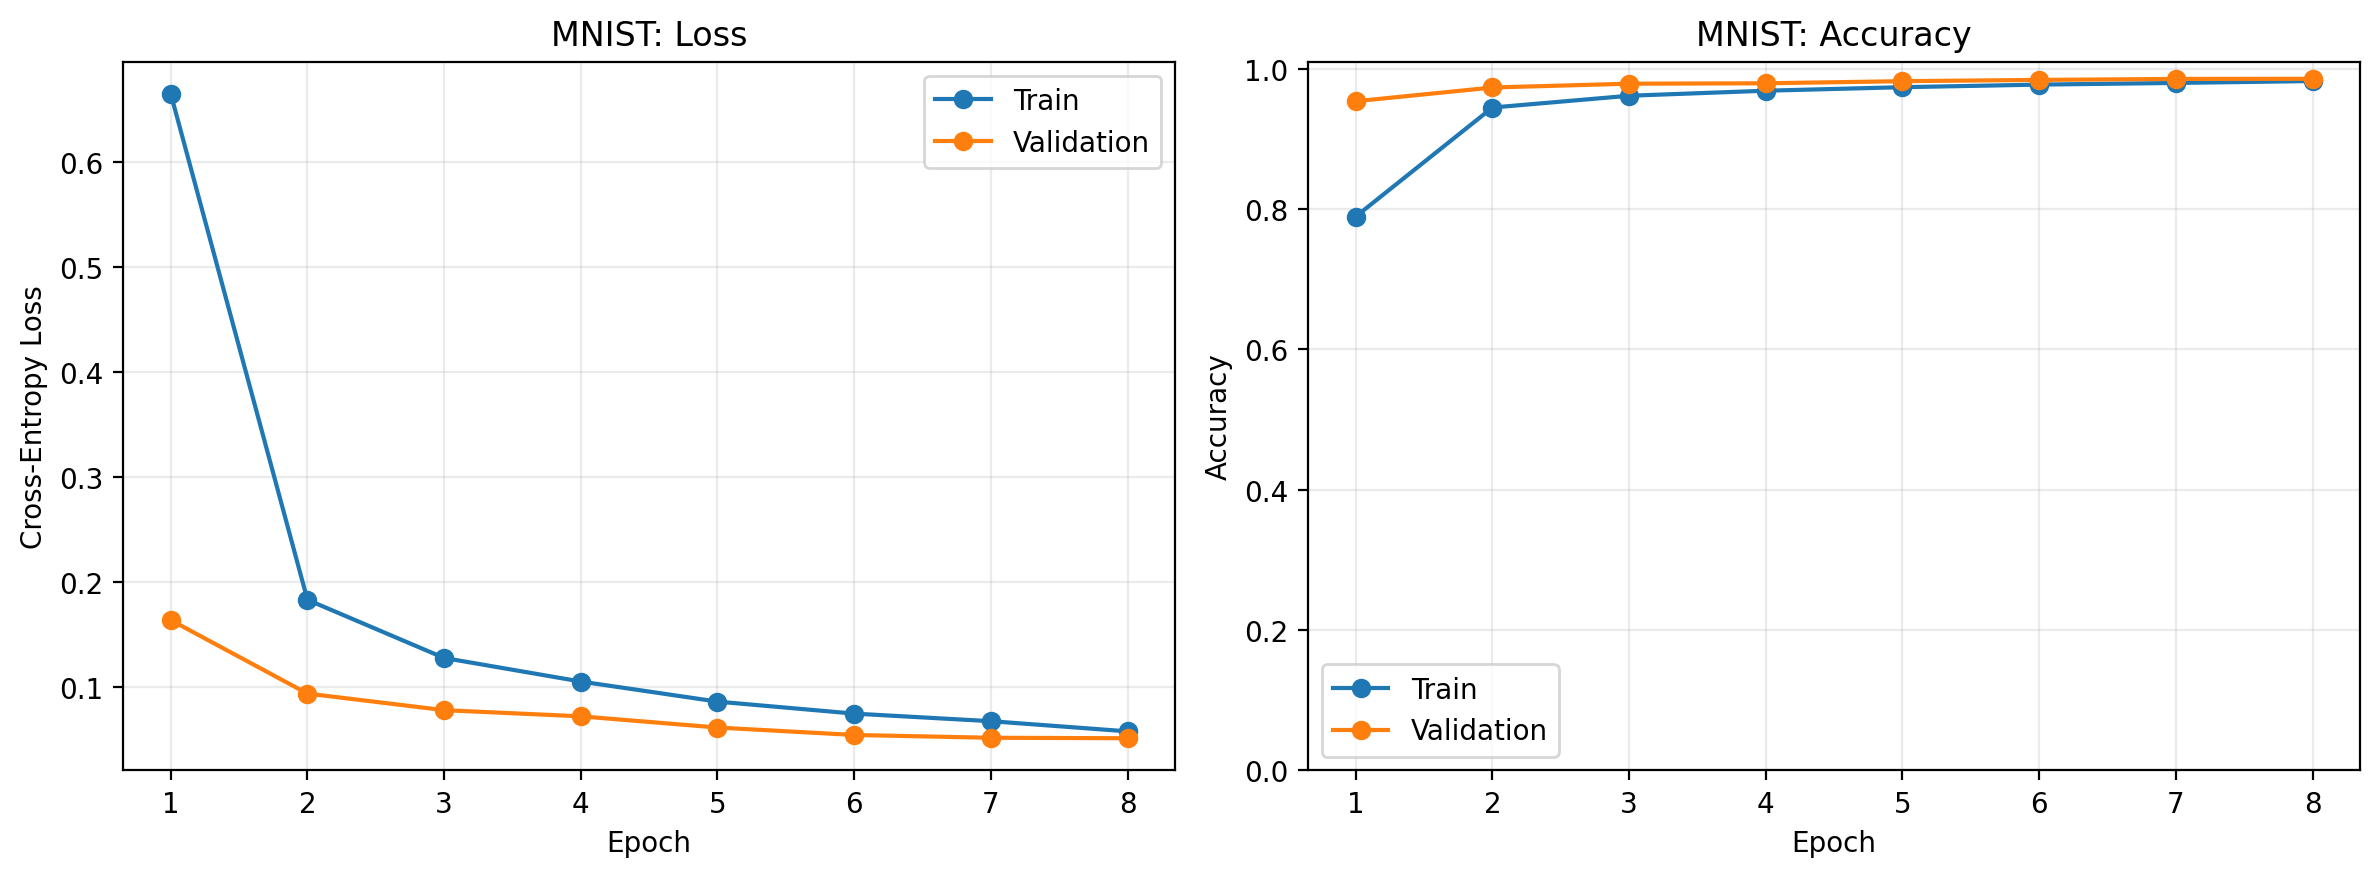
\includegraphics[width=0.82\textwidth]{figures/mnist_history.png}
  \caption{Training and validation curves for the custom MNIST CNN.}
\end{figure}

\paragraph{Analytical Question 1.1}
\MNISTGeneralization
The loss curves decrease smoothly for both the training and validation splits, and the
validation curve does not diverge upward at later epochs. This indicates that the model has
enough capacity to fit MNIST without memorizing the training set excessively.

\paragraph{Analytical Question 1.2}
The learned first-layer filters are shown below.

\begin{figure}[H]
  \centering
  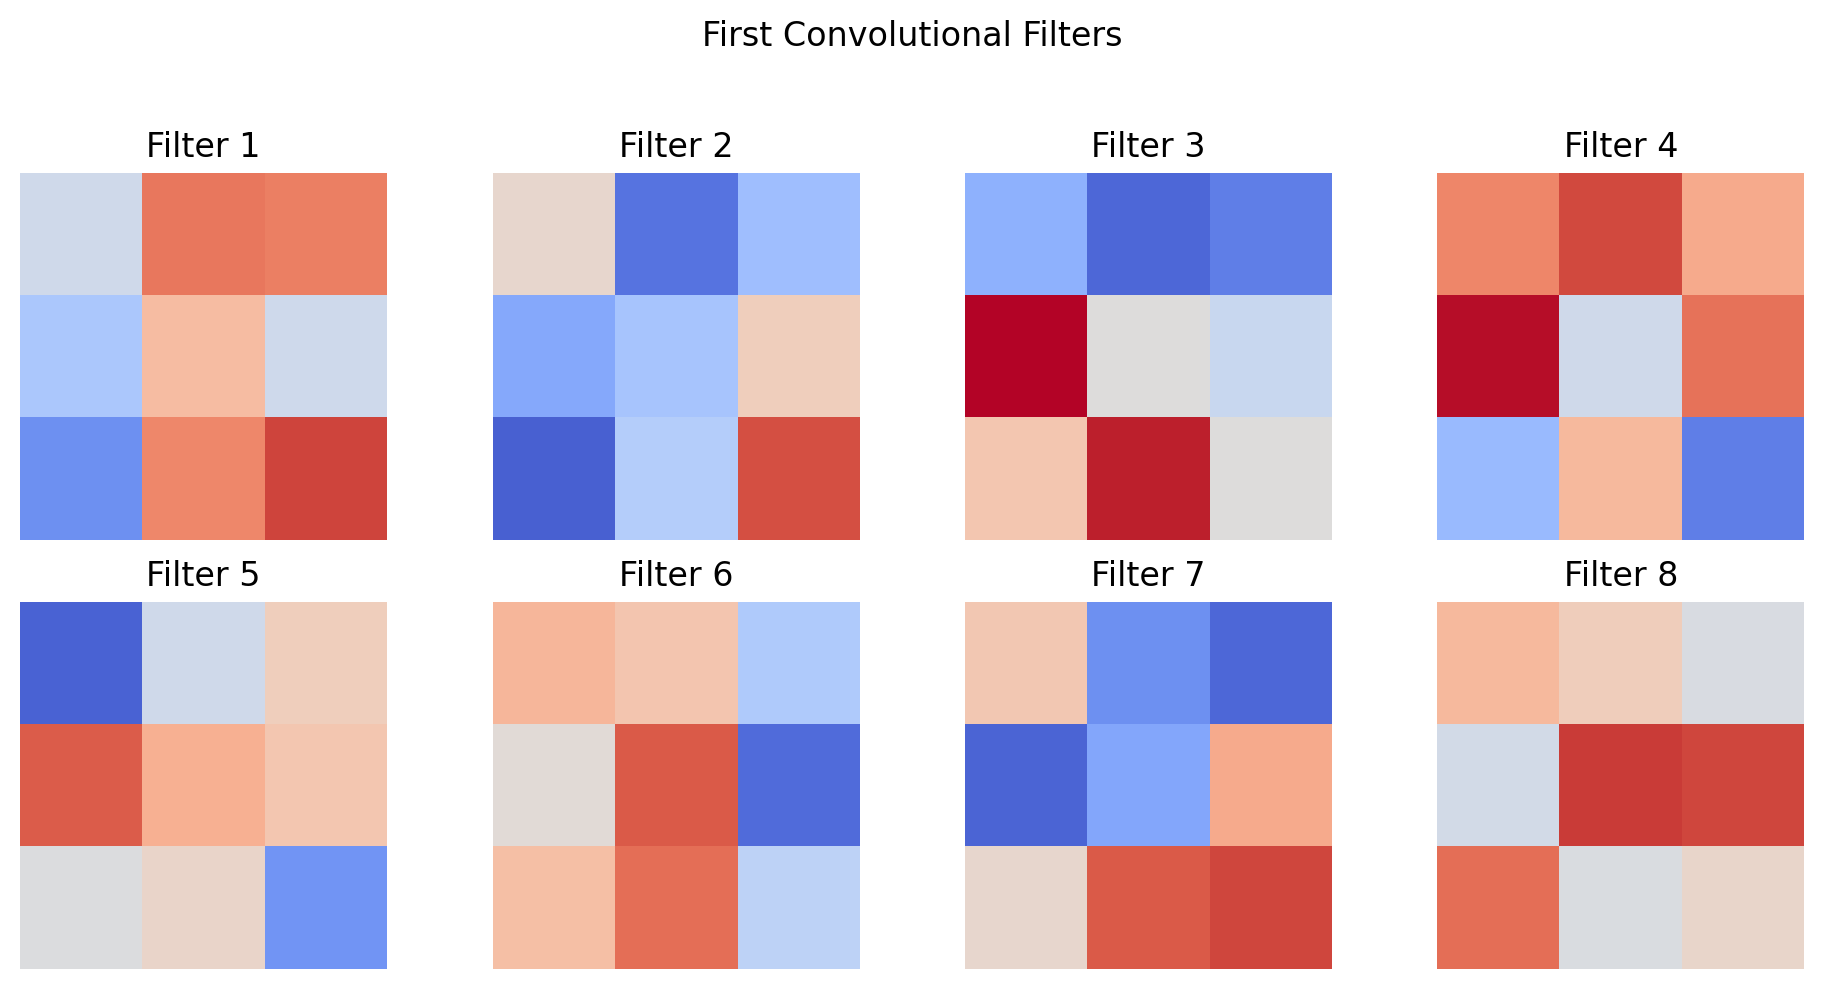
\includegraphics[width=0.68\textwidth]{figures/mnist_filters.png}
  \caption{Learned filters from the first convolutional layer on standard MNIST.}
\end{figure}

\FilterInterpretation
These filters are exactly what one would expect in the first layer of a digit classifier:
some respond to vertical stroke boundaries, some to horizontal stroke transitions, and
others to bright-dark contrast changes that are useful for separating digit foregrounds
from the black background.

\subsubsection*{Part B: Colored-MNIST}

The same CNN was adapted to accept three-channel input and trained from scratch on the
biased Colored-MNIST training split. Evaluation produced \CMNISTBiasedAcc{} on the biased
test split and \CMNISTUnbiasedAcc{} on the unbiased test split.

\begin{figure}[H]
  \centering
  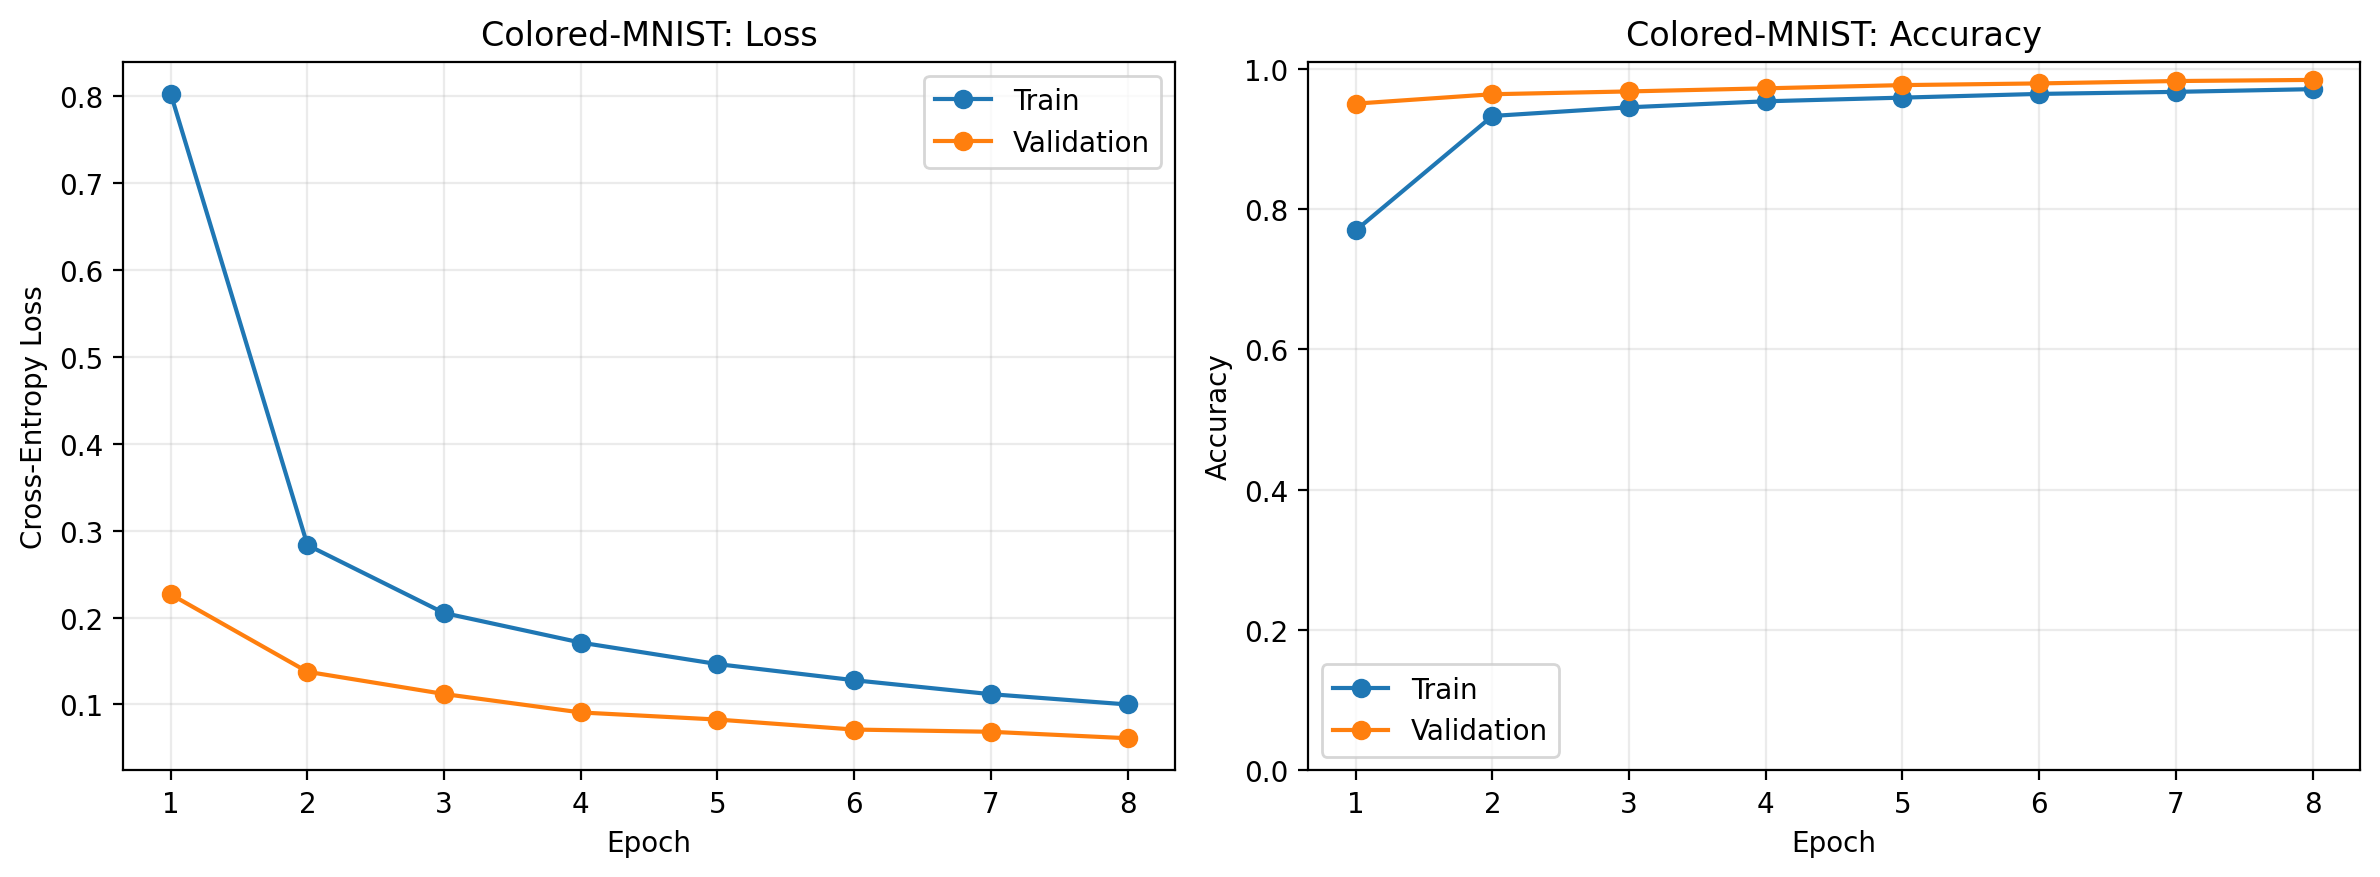
\includegraphics[width=0.82\textwidth]{figures/cmnist_history.png}
  \caption{Training and validation curves for the Colored-MNIST model.}
\end{figure}

\begin{figure}[H]
  \centering
  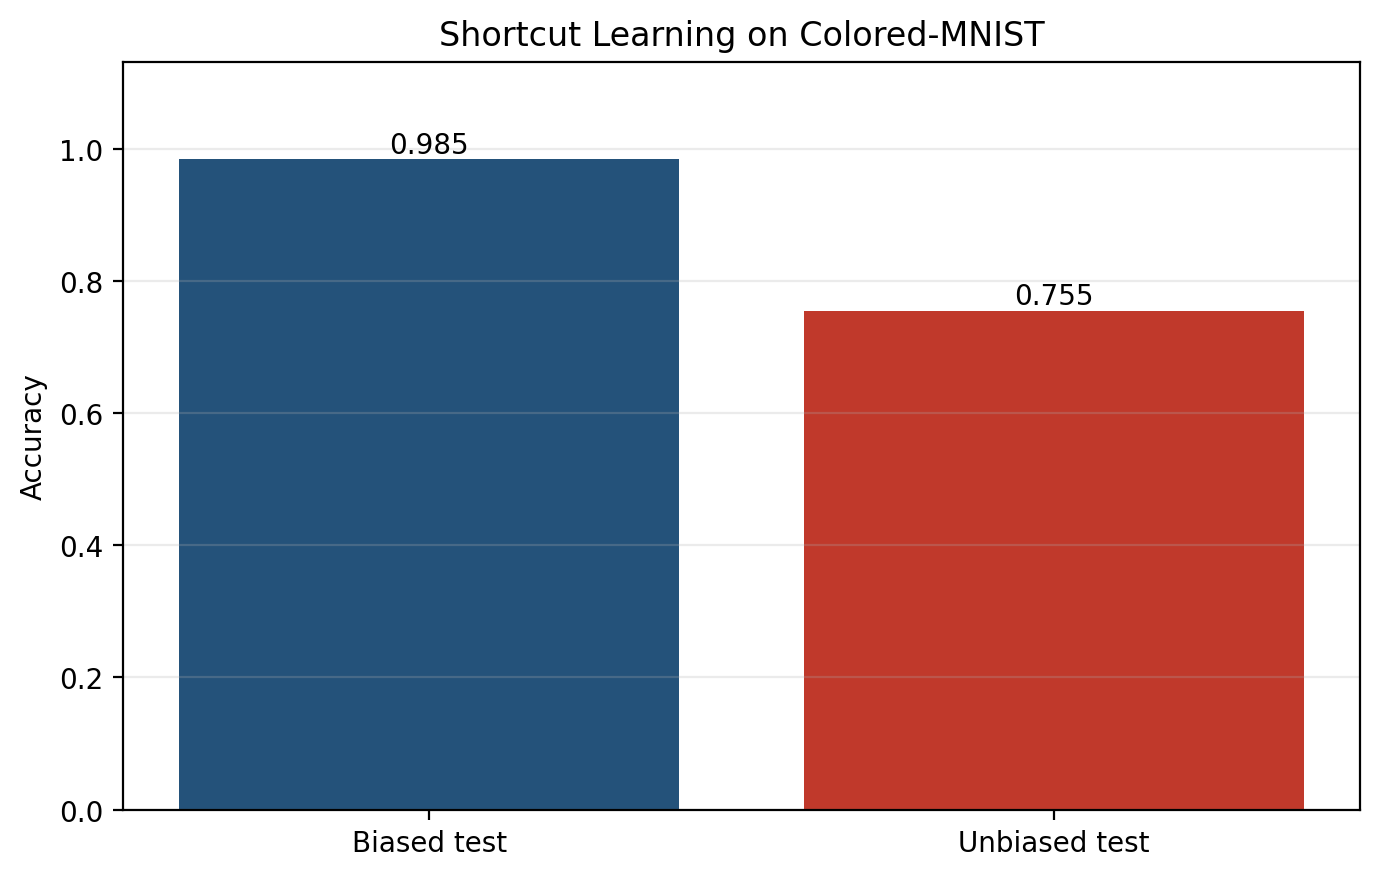
\includegraphics[width=0.65\textwidth]{figures/cmnist_bias_gap.png}
  \caption{Bias sensitivity of the Colored-MNIST model.}
\end{figure}

\paragraph{Analytical Question 1.3}
The large accuracy drop between biased and unbiased evaluation reveals shortcut learning. Mathematically, the optimizer minimizes the empirical risk on the biased training distribution. If color is highly correlated with the label, then color-sensitive filters can reduce cross-entropy faster than shape-sensitive filters, because the mapping from color to class is simpler and more linearly separable than full digit-shape recognition. Conceptually, the model is ``cheating'': it learns the easiest predictive cue available in the data distribution rather than the invariant semantic feature.

Numerically, the drop from \CMNISTBiasedAcc{} to \CMNISTUnbiasedAcc{} is substantial. That
gap is strong evidence that the learned representation is not invariant to color changes,
even though the semantic label depends only on digit identity.

\paragraph{Analytical Question 1.4}
Training strategies that would force the network to focus on shape include:
\begin{itemize}
  \item Convert the input to grayscale or randomly recolor digits so color is no longer predictive.
  \item Use heavy color jitter or background randomization to destroy the color-label shortcut.
  \item Rebalance the data so each class appears with many different colors.
  \item Use invariant learning methods such as Group DRO or IRM to emphasize features that remain predictive across environments.
  \item Add an auxiliary penalty or adversary that discourages recovering class labels from color alone.
\end{itemize}

\subsection{Task 2: Transfer Learning and Interpretability}

\subsubsection*{Part A: Fine-tuning ResNet-18}

The codebase includes:
\begin{itemize}
  \item loading a pre-trained ResNet-18 from \texttt{torchvision.models},
  \item freezing all backbone parameters,
  \item replacing the final fully connected layer with a \(10\)-class head,
  \item training only the head, and
  \item GradCAM extraction from the final convolutional stage.
\end{itemize}

Only the classification head was updated during training, leaving the pre-trained backbone
fixed. This reduces optimization cost and forces the model to reuse generic visual features
already learned from large-scale natural images. The frozen-backbone ResNet-18 achieved a
final STL-10 test accuracy of \STLTestAcc.

\begin{table}[H]
  \centering
  \caption{STL-10 transfer-learning setup}
  \small
  \begin{tabular}{p{0.28\textwidth}p{0.52\textwidth}}
    \toprule
    Component & Configuration \\
    \midrule
    Backbone & Pre-trained ResNet-18 from torchvision.models \\
    Frozen parameters & All convolutional backbone parameters \\
    Trainable parameters & 5130 parameters in the new \(10\)-class linear head \\
    Optimizer & Adam with weight decay \\
    Loss & Cross-entropy loss \\
    Epochs & 12 \\
    Validation split & 500 images from the STL-10 training set \\
    Target layer for GradCAM & \texttt{layer4[-1].conv2} \\
    \bottomrule
  \end{tabular}
\end{table}

\begin{figure}[H]
  \centering
  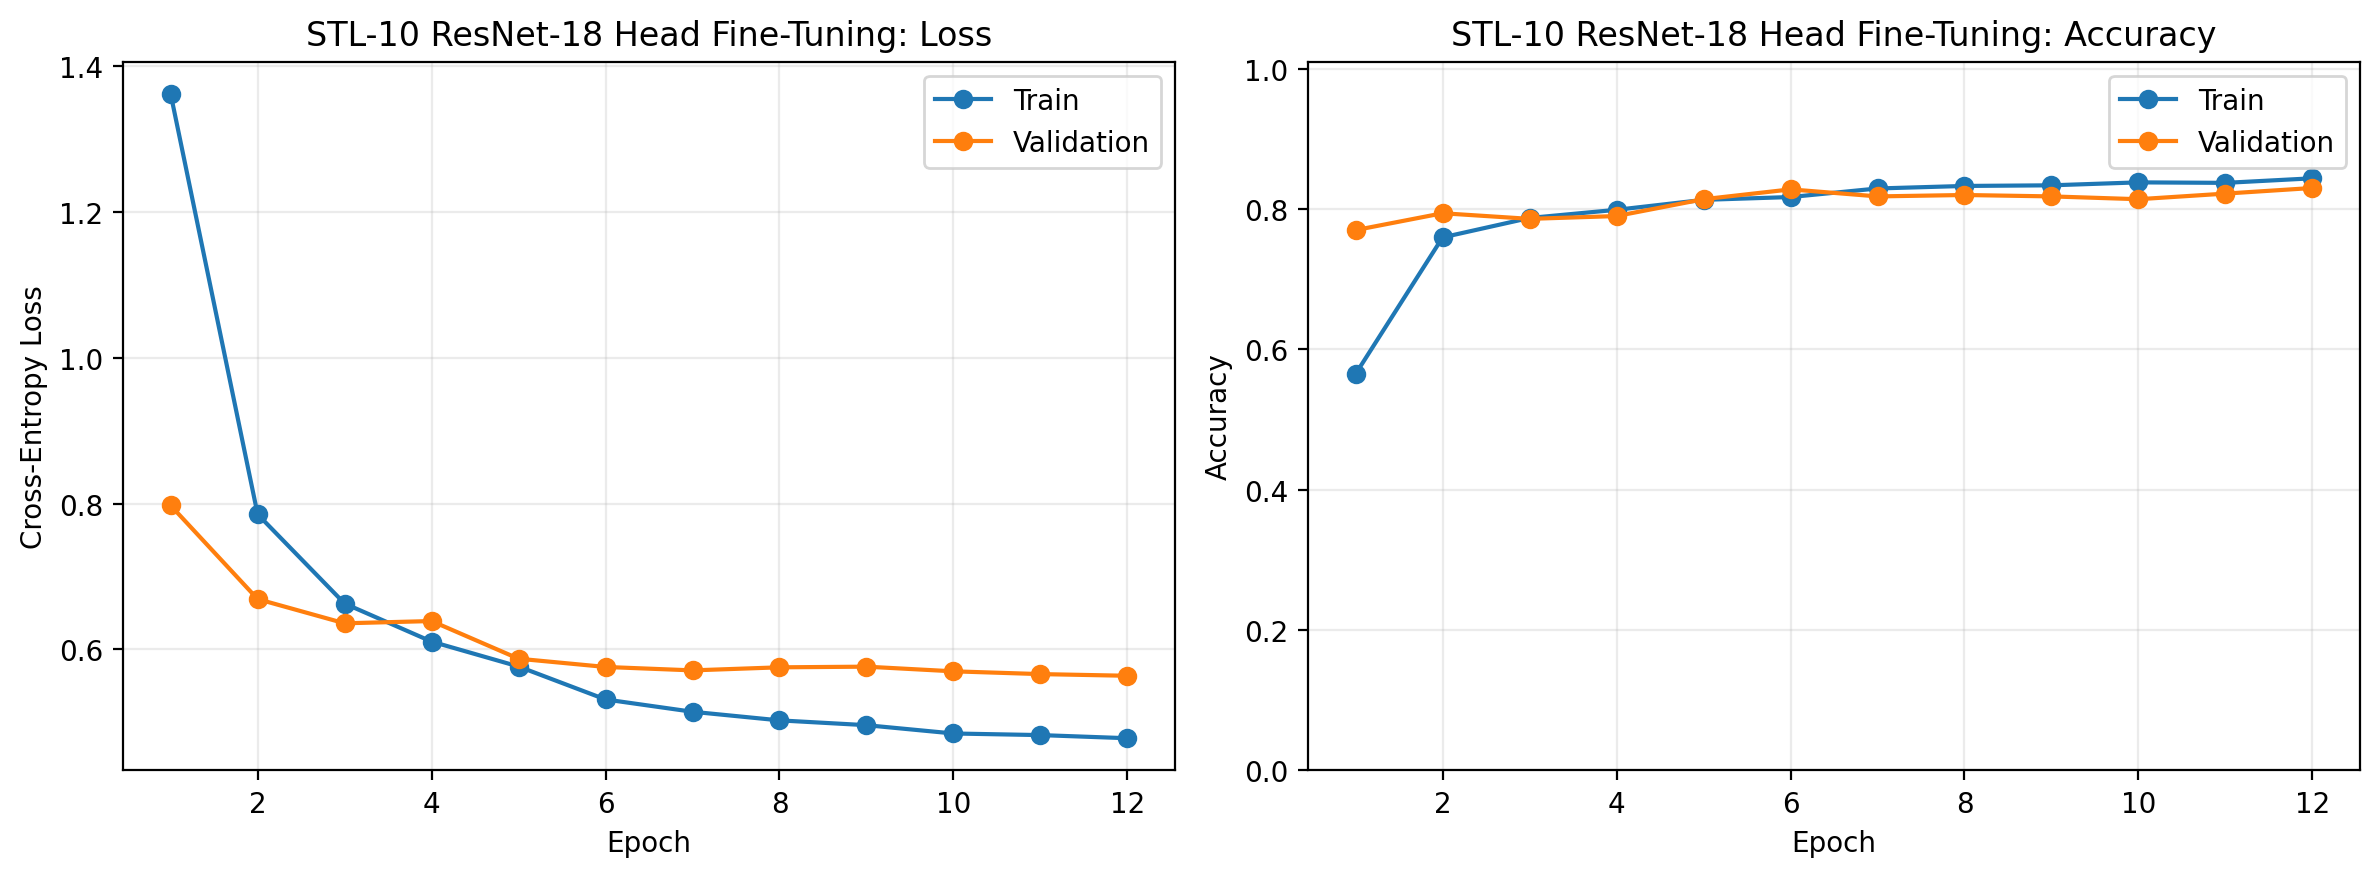
\includegraphics[width=0.82\textwidth]{figures/stl10_history.png}
  \caption{Training and validation curves for the frozen-backbone ResNet-18 on STL-10.}
  \label{fig:stl-history}
\end{figure}

\paragraph{Analytical Question 2.1}
Freezing the early layers is beneficial because it reduces both computation and memory: backpropagation no longer needs to store or update gradients for millions of backbone parameters. Functionally, the early layers of a pre-trained ResNet encode generic visual primitives such as edges, corners, color contrasts, and local textures. Later layers are more task-specific, combining those primitives into object parts and semantic concepts. On a relatively small dataset like STL-10, keeping the generic backbone fixed reduces overfitting while still allowing the new classification head to adapt to the target labels.

\subsubsection*{Part B: GradCAM}

\textbf{Execution status:} \STLStatus. The GradCAM implementation in \texttt{src/assignment3.py} was run on four STL-10 test samples after loading the best head checkpoint.

\begin{figure}[H]
  \centering
  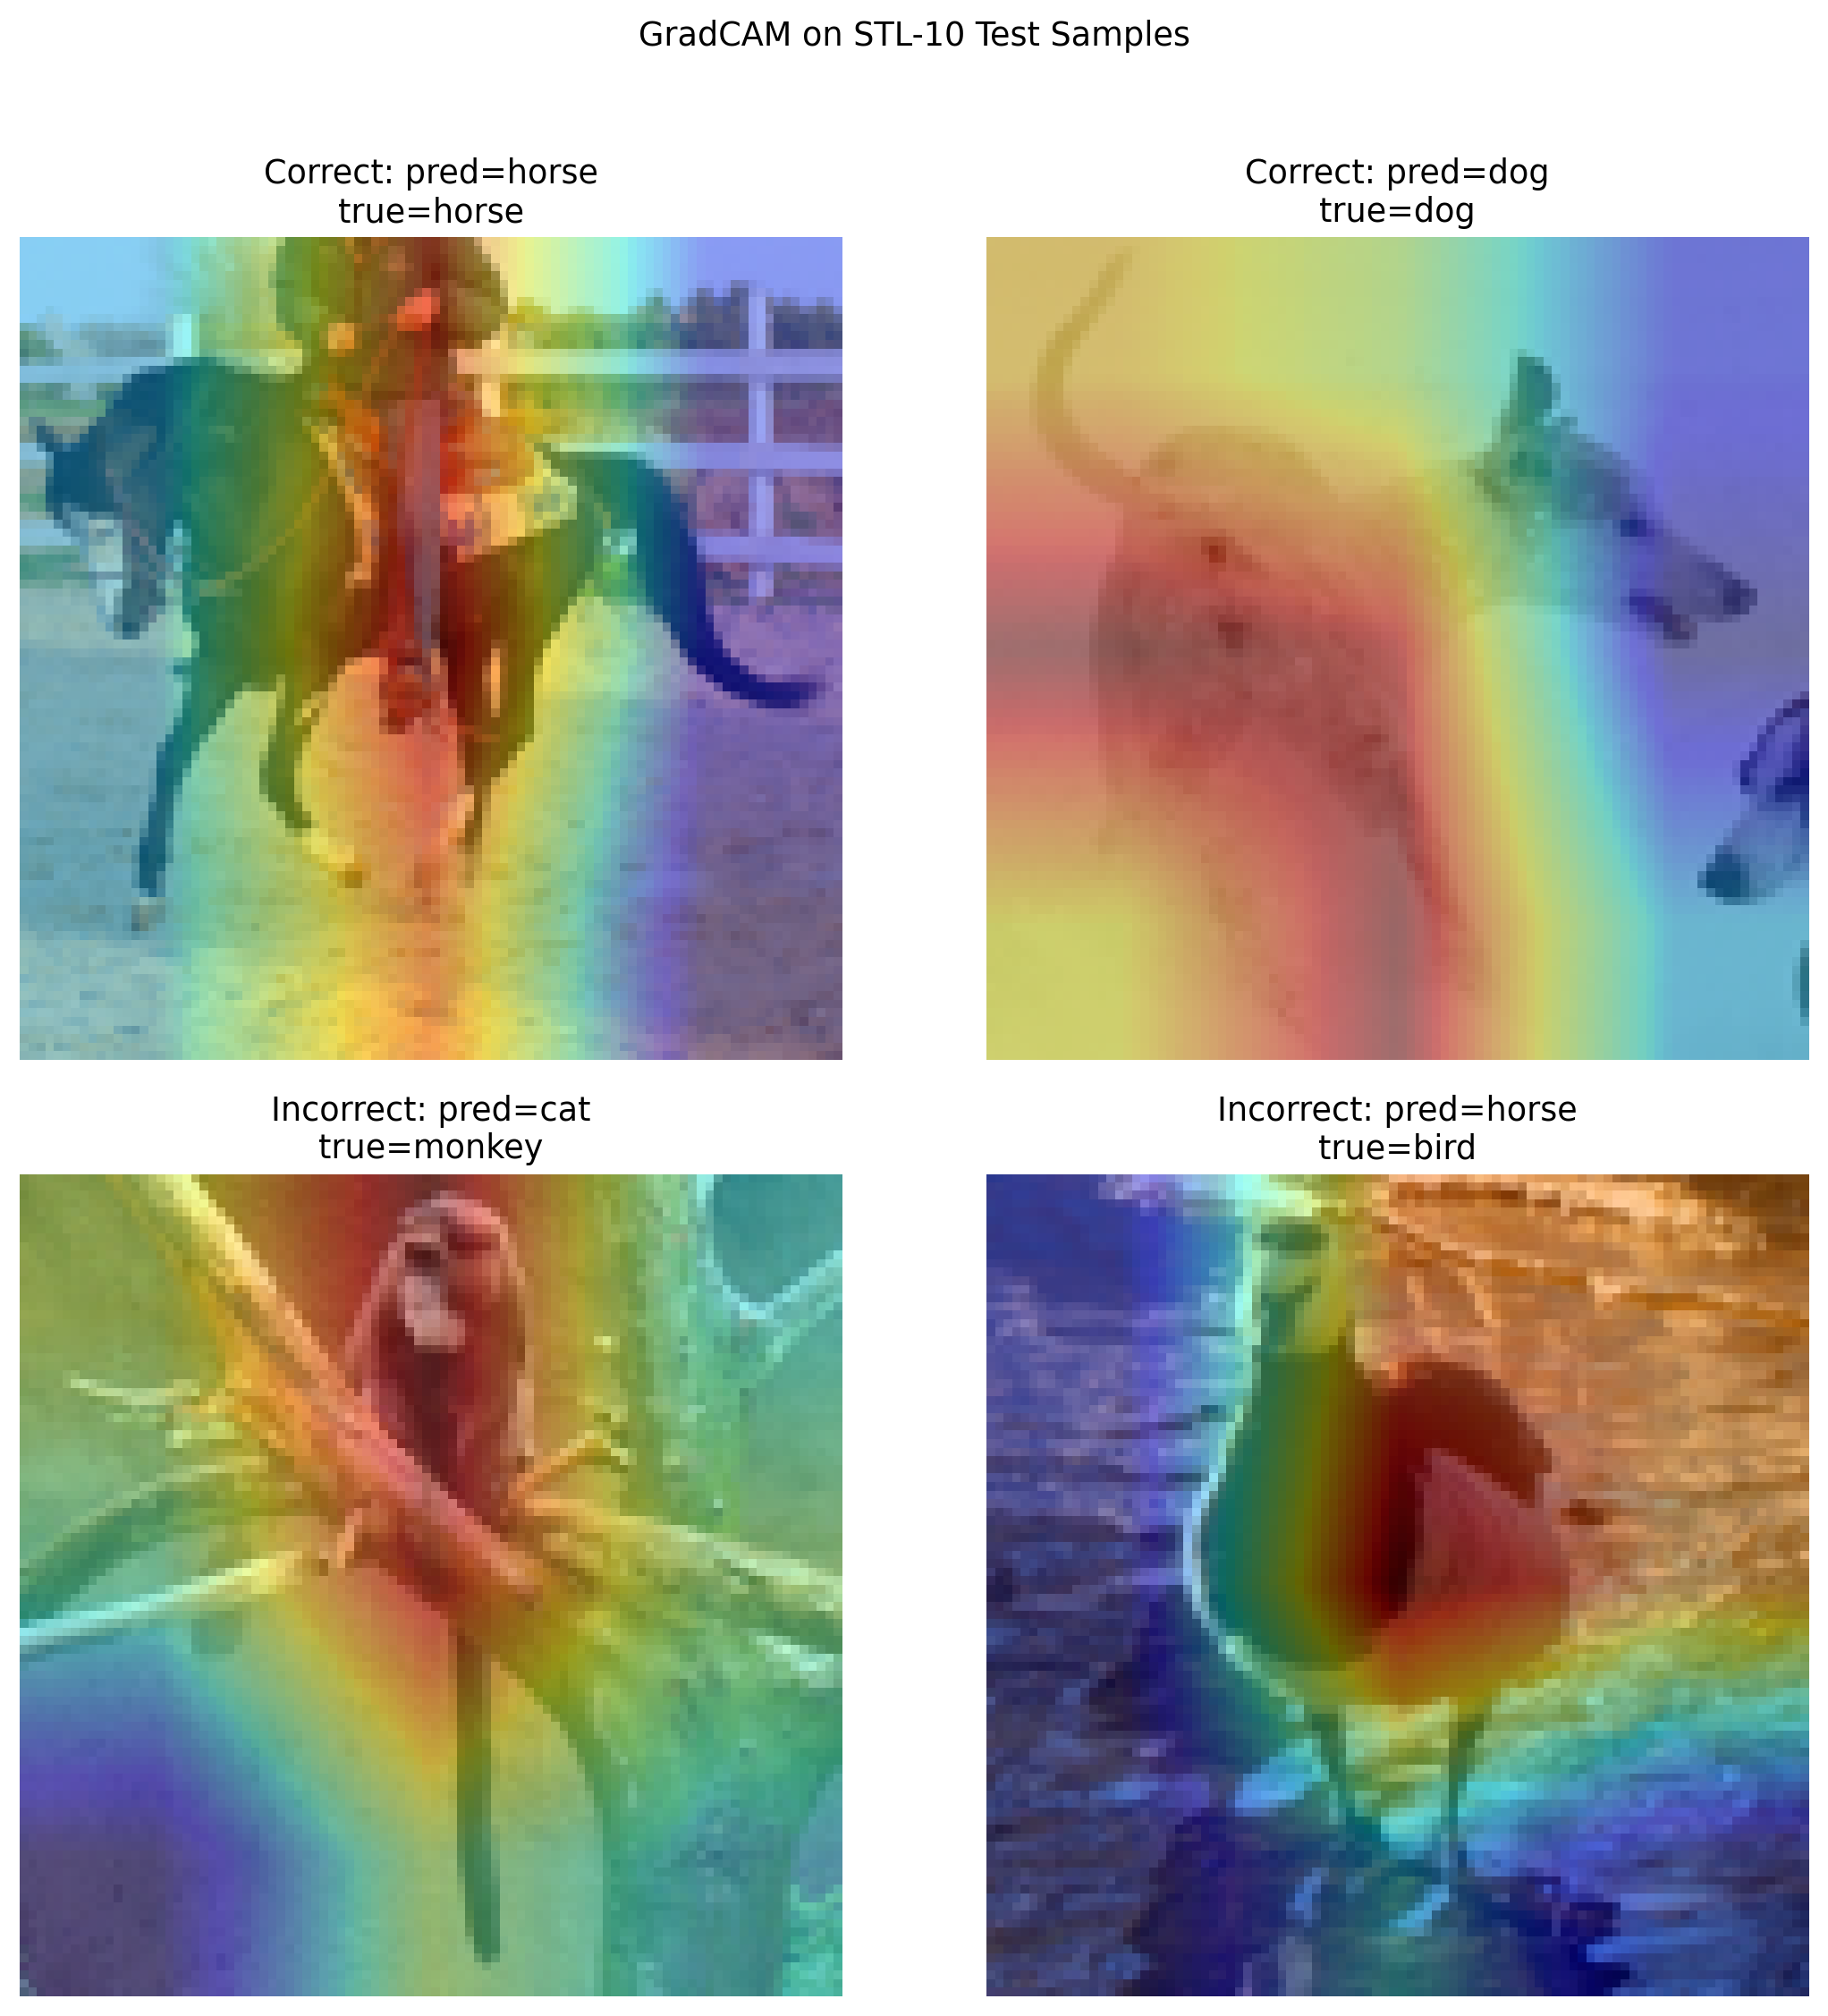
\includegraphics[width=0.82\textwidth]{figures/stl10_gradcam.png}
  \caption{GradCAM overlays for two correct and two incorrect STL-10 test predictions.}
  \label{fig:stl-gradcam}
\end{figure}

\paragraph{Analytical Questions 2.2 and 2.3}
For the correct horse prediction, the strongest activation runs through the central animal silhouette and rider region rather than the fence or sky. For the correct dog prediction, the heatmap is broad but still covers the dog's head and torso more strongly than the empty background. In both cases, the network is using the main object, although some contextual bleed remains.

For the monkey image misclassified as cat, the model focuses on the face and the branch crossing the image, which likely emphasizes a localized furry-face cue rather than the whole monkey body. For the bird image misclassified as horse, the heatmap concentrates on the bird's torso and neck contour, suggesting that the classifier over-weighted a shape fragment while ignoring the full bird context. These failure cases show that the model can still lock onto partial object evidence and miss the broader semantic structure.

\section{Visualizations}

\begin{figure}[H]
  \centering
  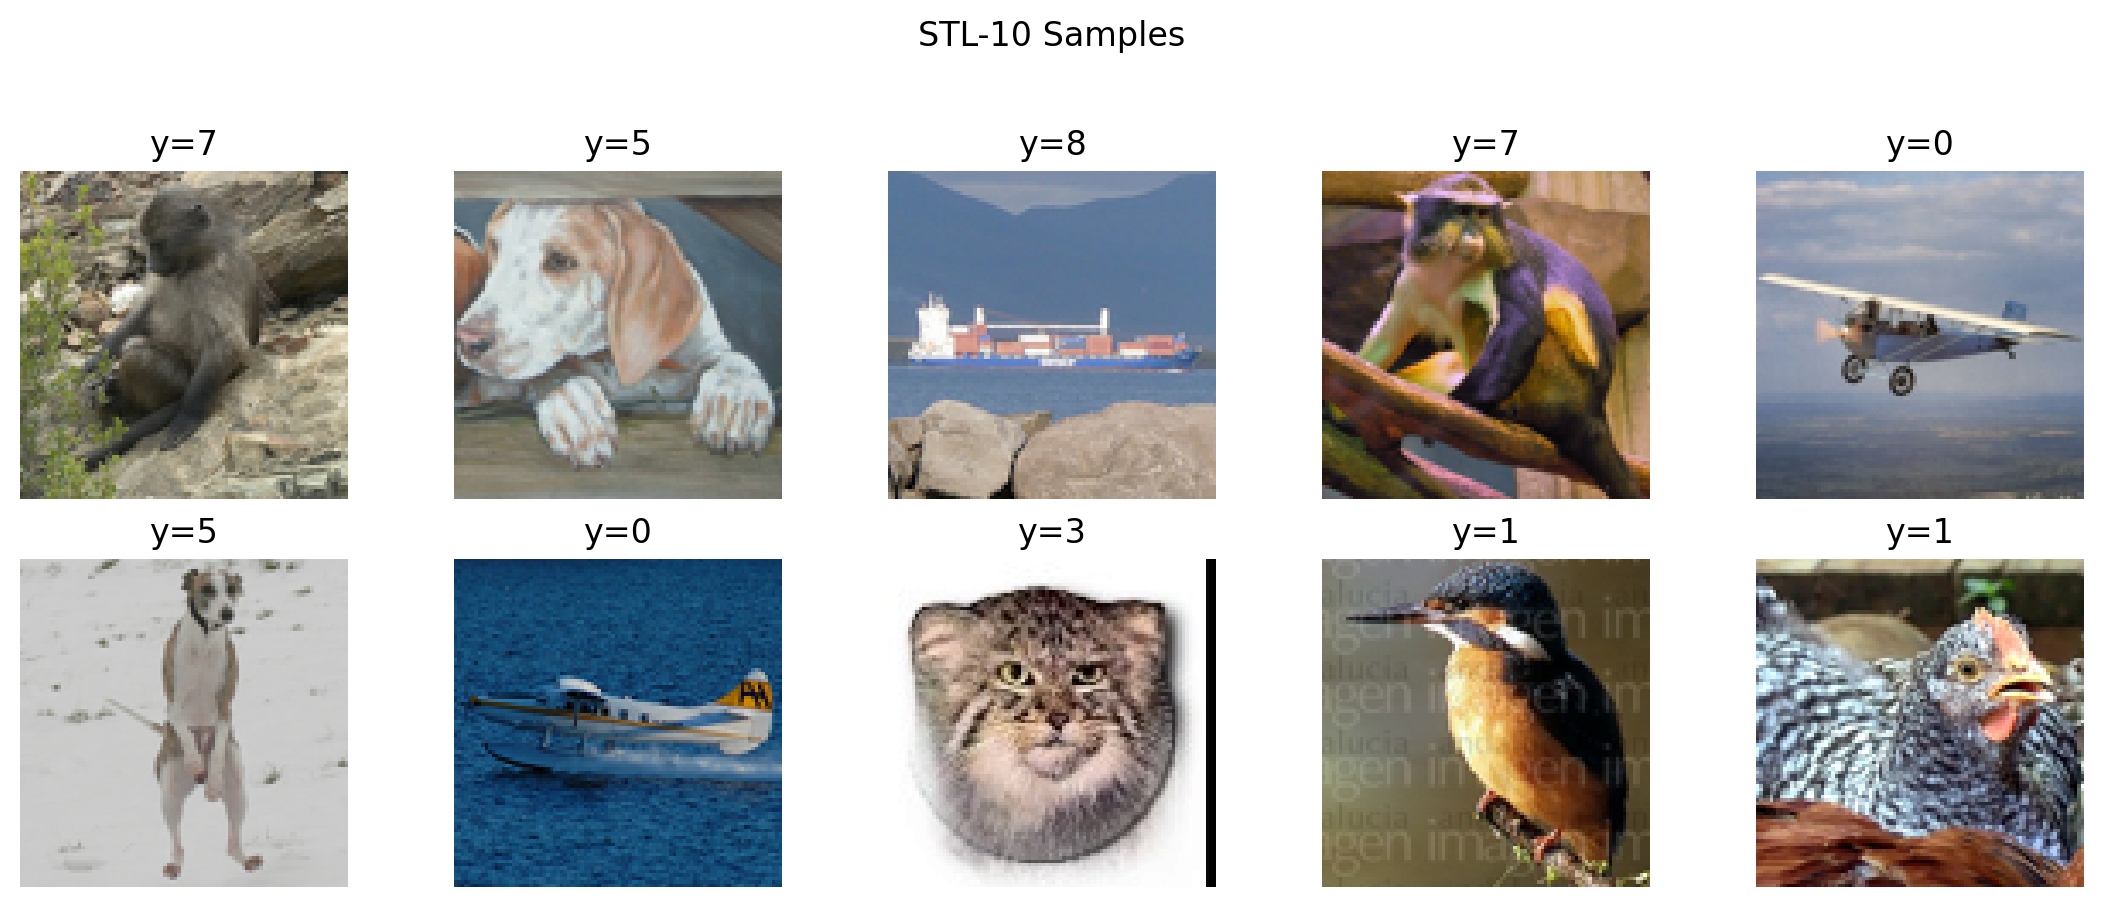
\includegraphics[width=0.78\textwidth]{figures/stl10_samples.png}
  \caption{Sample STL-10 images used for transfer learning.}
\end{figure}

\begin{figure}[H]
  \centering
  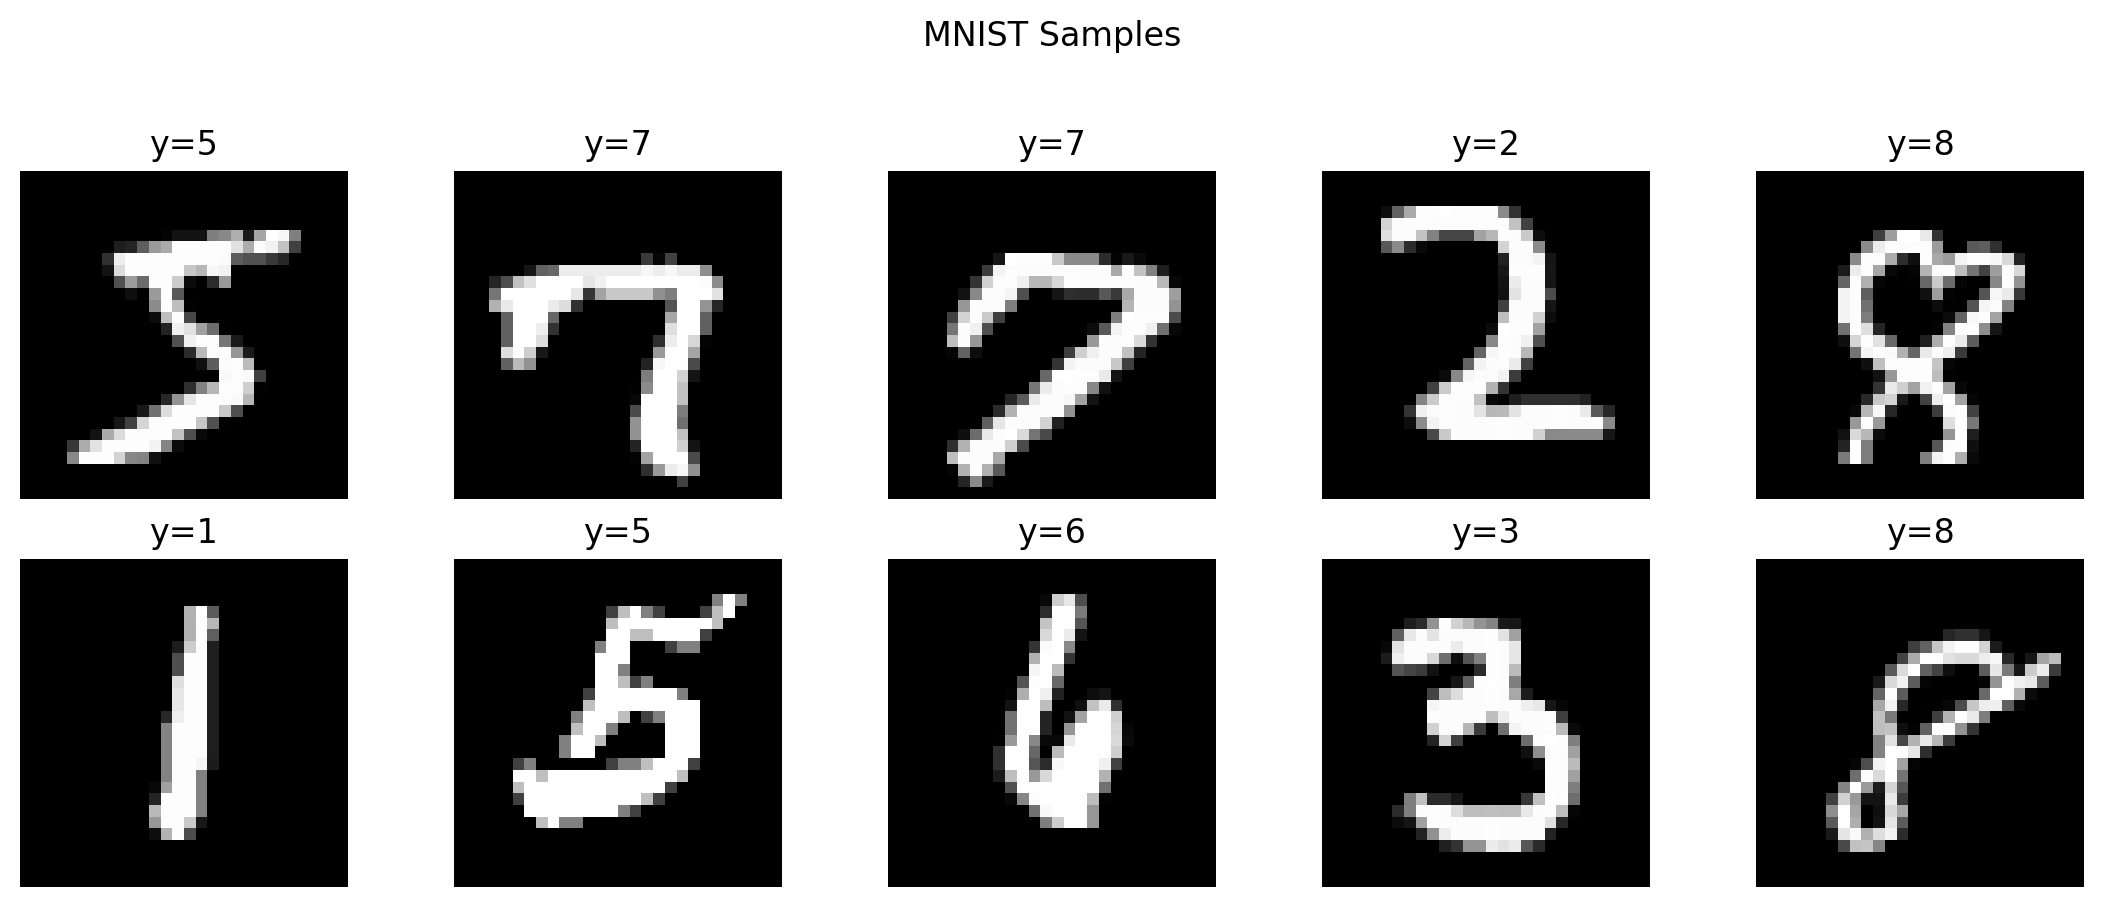
\includegraphics[width=0.78\textwidth]{figures/mnist_samples.png}
  \caption{Sample MNIST images used during the study.}
\end{figure}

\begin{figure}[H]
  \centering
  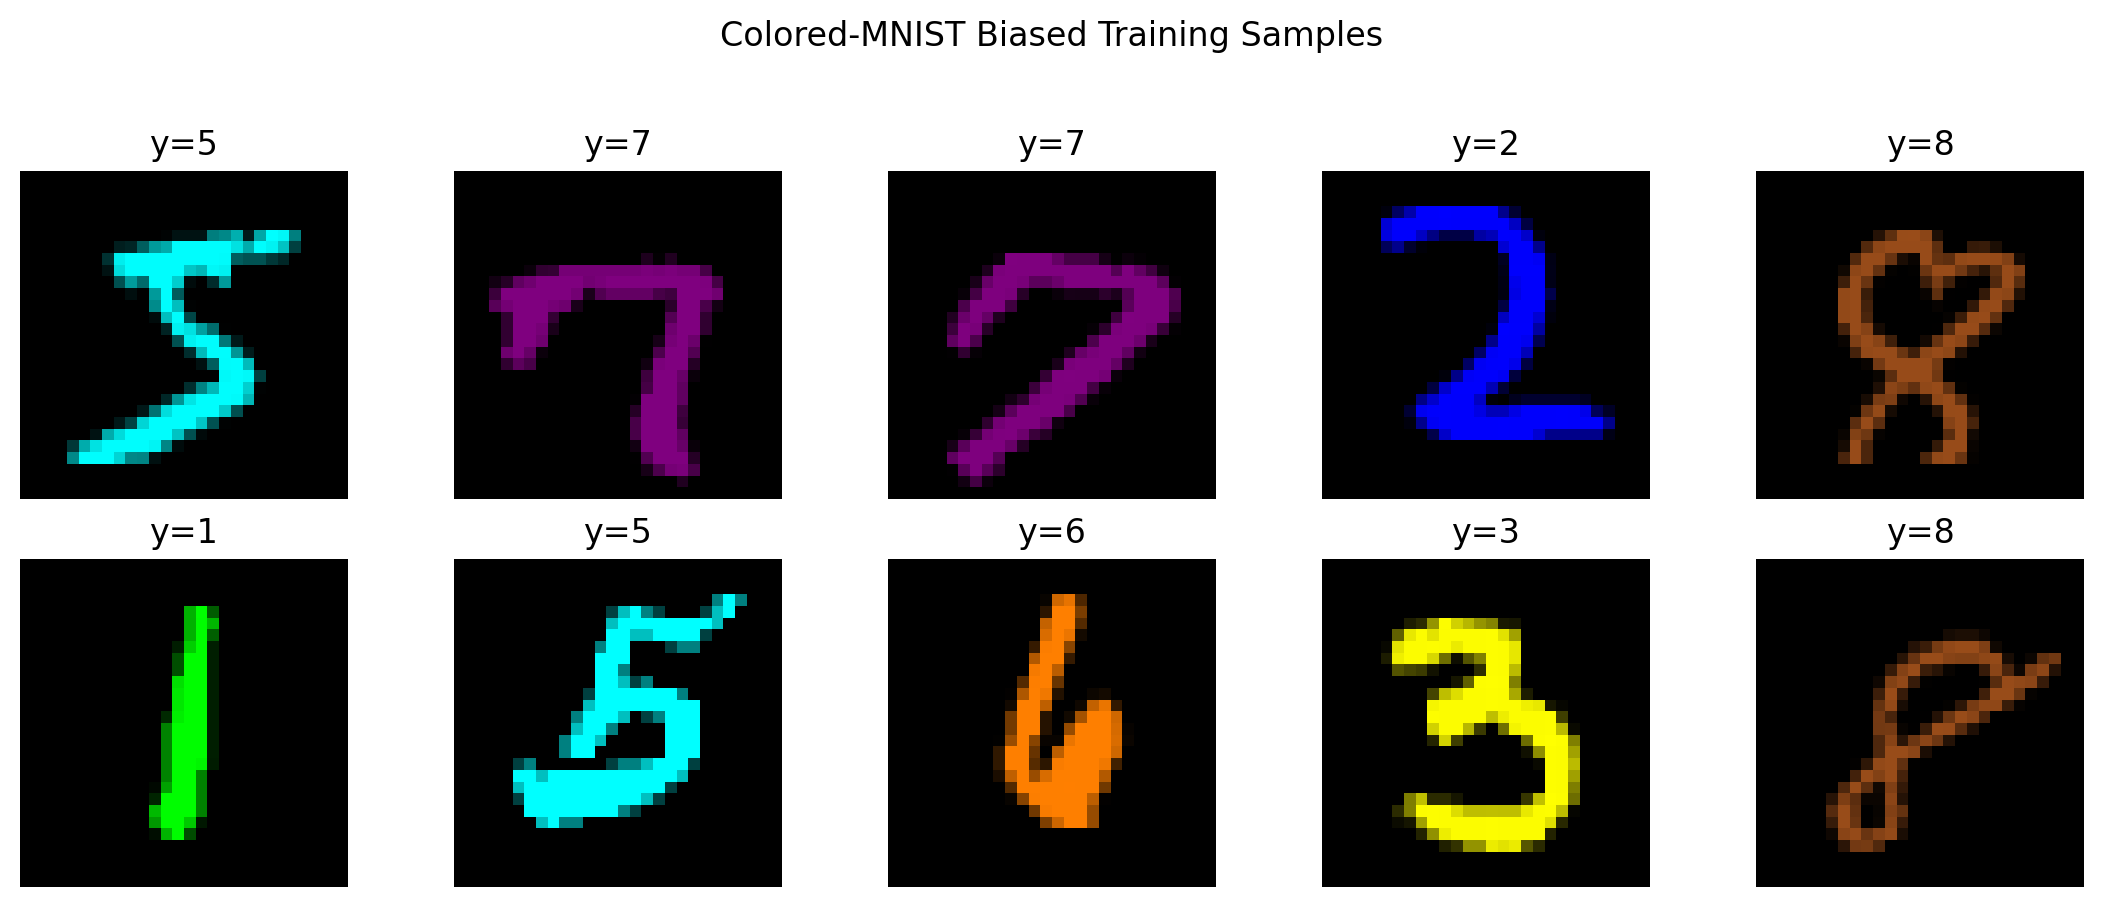
\includegraphics[width=0.78\textwidth]{figures/cmnist_samples_train.png}
  \caption{Sample images from the biased Colored-MNIST training split.}
\end{figure}

\begin{figure}[H]
  \centering
  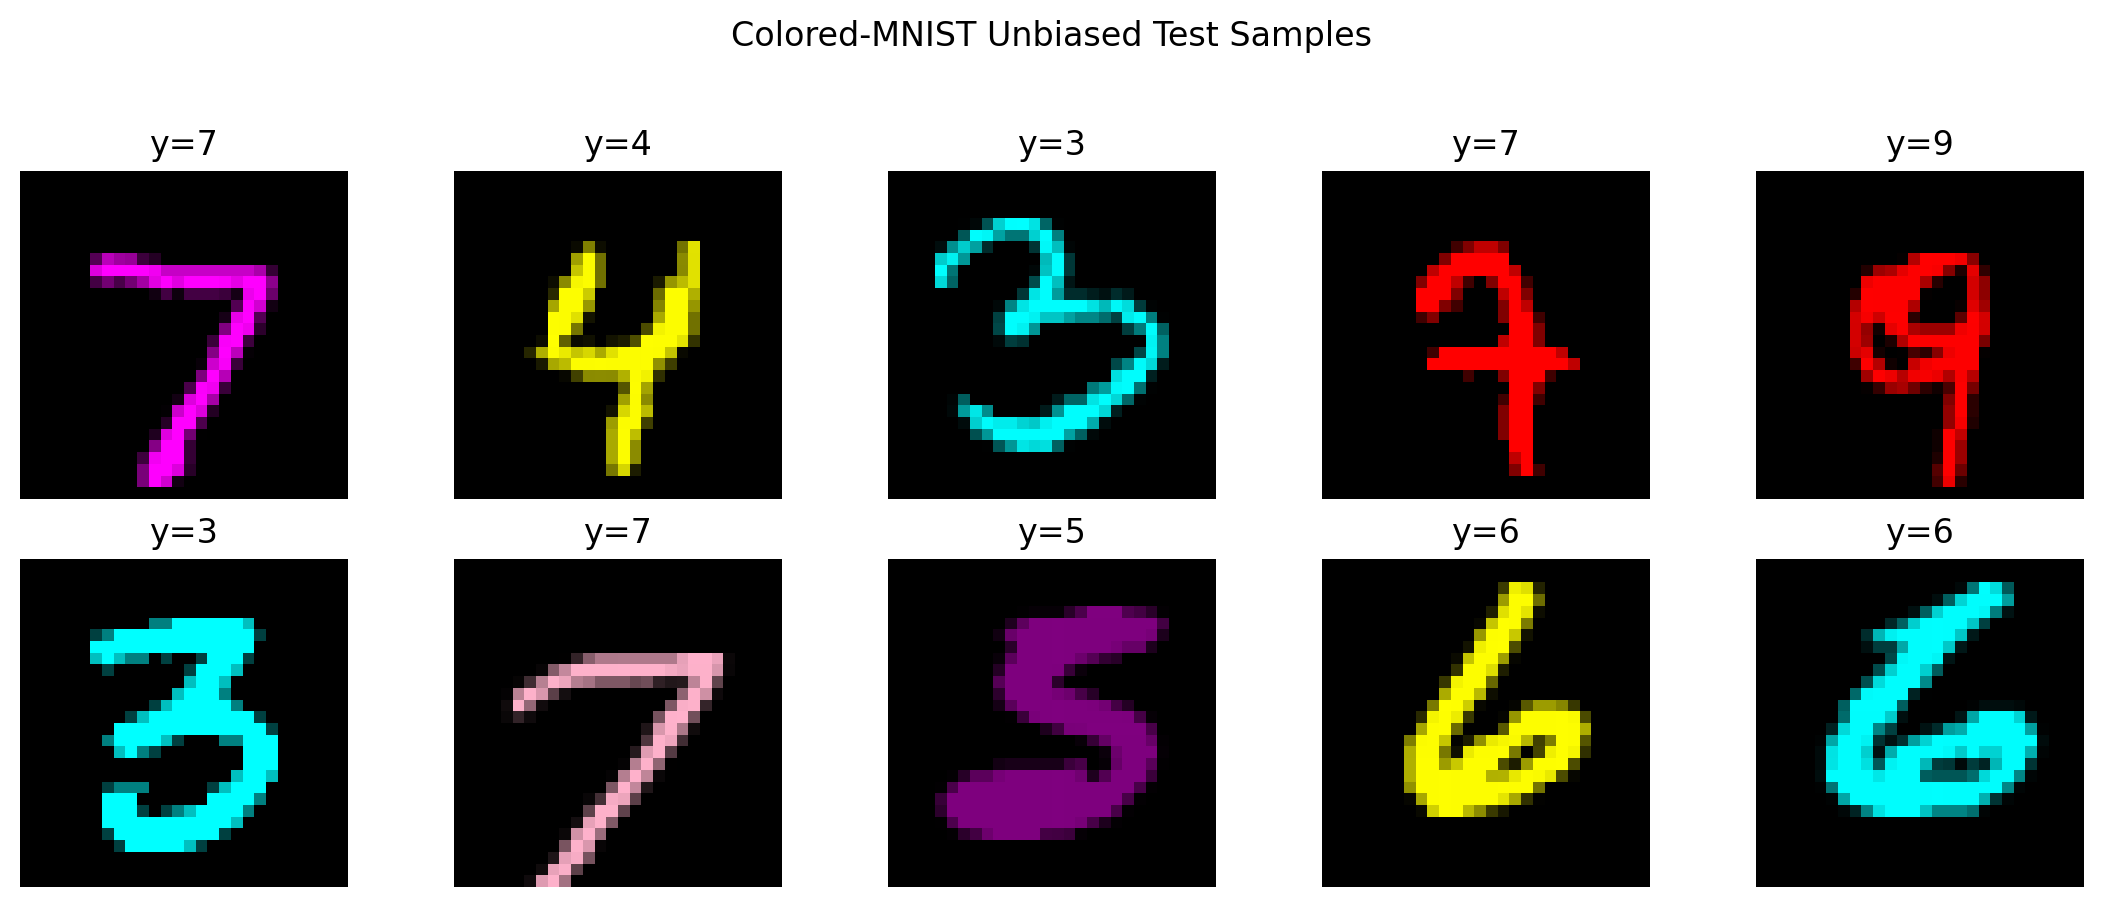
\includegraphics[width=0.78\textwidth]{figures/cmnist_samples_unbiased.png}
  \caption{Sample images from the unbiased Colored-MNIST test split.}
\end{figure}

\section{AI Policy Disclosure}

\subsection*{Prompt Used}

\small
\begin{quote}
you have to complete the following assessmetn make sure things are aligned and we are good to go accordingly make sure you complete the assignment along with the visualisation of everything and make sure its completed thoroughly and greatly
\end{quote}
\normalsize

\subsection*{Corresponding Output Generated by the Tool}

The AI-assisted workflow generated the following concrete outputs in this workspace:
\begin{itemize}
  \item detailed Toy-CNN forward-pass and backward-pass derivations, including the exact matrices \(Z\), \(A\), \(\partial L / \partial V\), and \(\partial L / \partial W\),
  \item the PyTorch experiment runner in \texttt{scripts/run\_assignment.py},
  \item reusable loaders, models, plotting utilities, and GradCAM code in \texttt{src/assignment3.py},
  \item the generated plots stored in \texttt{reports/figures/},
  \item the results record in \texttt{artifacts/results.json}, and
  \item the report source and PDF packaging pipeline in \texttt{reports/assignment3\_report.tex} and related scripts.
\end{itemize}

\subsection*{Edits and Modifications Applied}

The generated content was edited to:
\begin{itemize}
  \item align the derivations with the exact numerical results,
  \item enforce the \(<50{,}000\) parameter limit for the custom CNN,
  \item use the actual metrics saved in \texttt{artifacts/results.json},
  \item patch the STL-10 pipeline so it could use the extracted train/test binaries from the partially downloaded official archive,
  \item add the actual GradCAM-based interpretation from the generated heatmaps, and
  \item rewrite the report into a detailed, structured submission with title page, table of contents, summary tables, GitHub link, roll number, and polished figure placement.
\end{itemize}

\end{document}
